% Body of the MMM 2027 submission. Edit this file directly.

\section{Introduction}


A moving object supplies photometric and geometric residuals that a rigid-world estimator resolves by moving the camera. Run unmodified, our 3DGS-SLAM backbone drifts to 39.3 cm on the mixed-mover sequence \texttt{balloon} and 147.5 cm on a crowded one, against roughly 1.5 cm on static scenes. The input is handheld RGB-D video, and it arrives full of uncontrolled content such as balloons, carried boxes, and objects placed and removed. The dominant response detects the movers and removes them. An external, class-conditioned network labels which pixels could move, and the estimator discards them (Sec. 2.1). This works, but it makes the dynamic decision a per-frame classification by a second model, with its cost and failure modes. It is also closed-set, which bites hardest on user-generated content, where the label set is open. Recent lines replace the \emph{class} prior with a learned uncertainty (Sec. 2.2) or move the decision out of the segmentation network (Sec. 2.3).


Our configuration sits in that third line. It decides which pixels to trust from \emph{consistency}, the disagreement between observed optical flow and the flow a rigid scene would produce, and it down-weights rather than removes. Operating without semantic segmentation is not itself a contribution we claim, since prior work has done that. Two kinds of evidence are missing. One shows which of its parts are necessary, and on which sequences. The other separates the mechanism's own effect from the extra information a method was handed.


We present RoGS-SLAM, a mask-free core for dynamic 3DGS-SLAM. On the crowd scenes it tracks at 2.2--2.3 cm where the backbone drifts to 86--147 cm, at 4.0 GB of GPU memory, and its mask-free core needs no category label. Its contributions are the measurements that bound this result:


\begin{enumerate}\setlength{\itemsep}{0pt}
\item \textbf{Component necessity is regime-dependent, and we measured it rather than asserting it.} A pre-registered three-factor factorial (8 cells $\times$ 5 sequences $\times$ 3 seeds = 120 runs) finds that uniform keyframe coverage is strongly positive on object-only sequences but negative on the two hardest. Robust reweighting is within seed noise on 3 of 5 sequences yet is the single largest effect on \texttt{balloon}. The reliability signal is the only component never negative anywhere (5 of 5, 3 cells directional). No sequence demonstrably rewards all three (0 of 5), so the full bundle is nowhere strictly necessary (Sec. 5.2). The useful subset is a function of the regime.

\item \textbf{The gain is not attributable to the information alone.} Under an equal, strictly causal budget on the byte-identical frozen flow, a naive per-pixel threshold stably improves on the baseline on only 2 of 4 held-out sequences and is worse on \texttt{pt2} (51.07 vs 45.37 cm). Our mechanism improves on 4 of 4 (1.63--4.99$\times$) and beats the naive counterpart on all four (Sec. 5.4), closing the ``it just had more information'' reading.

\item \textbf{The pose-side mechanism is a variance--bias trade, measured on the intermediate quantity.} One single-variable intervention, extending the semantic hard tracking mask of the \emph{combined} configuration from 10 to all 100 tracking iterations, moves the per-frame dynamic penalty worse (+0.0806 cm, 1.22$\times$ its noise floor) yet full-trajectory error better ($-$1.42 cm, 4.0$\times$). This rests on one sequence with two legs near their floors (Sec. 5.6). The consequence generalises beyond this system. A pose-side claim must name its endpoint.
\end{enumerate}


The same evidence delimits where the mask-free configuration is not sufficient (Sec. 5.5). We claim no state-of-the-art accuracy, and our full 18-sequence runs include the four sequences where both arms regress against the backbone (Sec. 6).




\section{Related Work}


\subsection{Dynamic SLAM built on explicit dynamic priors}


Dynamic SLAM has long followed \emph{detect-then-exclude}. DynaSLAM~\cite{dynaslam} computes a per-pixel segmentation with Mask R-CNN~\cite{maskrcnn}, NGD-SLAM~\cite{ngdslam} uses a YOLO detector, and RoDyn-SLAM~\cite{rodynslam} fuses flow and segmentation masks. The pattern is widespread in 3DGS dynamic SLAM. RGD-SLAM~\cite{rgdslam} segments with a pre-trained OneFormer, DG-SLAM~\cite{dgslam} initialises poses from DROID-VO~\cite{droidslam}, and BDGS-SLAM~\cite{bdgsslam}, DAGS-SLAM~\cite{dagsslam} and DynaGSLAM~\cite{dynagslam} build per-Gaussian dynamic priors from YOLO or SAM2~\cite{sam2} detections. In every case the dynamic decision is delegated to an external, class-conditioned model, with the costs named in Sec. 1.


\subsection{Replacing the class prior with a learned uncertainty}


WildGS-SLAM~\cite{wildgsslam} drops the category prior while keeping a learned one. It predicts per-pixel uncertainty from ``a pre-trained DINOv2 feature extractor'' and metric depth ``as estimated by Metric3D v2''. Its own overview defines \emph{Prior Free} as ``not using class priors''. We apply the same standard to ourselves. Our label is \emph{mask-free}, never \emph{prior-free}, and it, too, keeps a pretrained network (the frozen RAFT flow of Sec. 3.4).


\subsection{Dynamic decisions from consistency rather than from categories}


A third line keeps a segmentation or depth network but moves the dynamic decision out of it, with pre-3DGS roots. ReFusion~\cite{bonn} rejects dynamic residual pixels in a purely geometric RGB-D pipeline with no learned prior at all. Recent 3DGS systems refine the same move with learned front ends. Gassidy~\cite{gassidy} separates objects through the YOLO instance masks, then decides which are dynamic by analysing rendering-loss flows, so the category label never decides motion. DGS-SLAM~\cite{dgsslamkong} runs an online Track-Anything segmentation with a photometric-consistency mask. Dy3DGS-SLAM~\cite{dy3dgsslam} fuses an optical-flow mask with a depth mask from ``the DepthanythingV2 estimation network''. GARAD-SLAM~\cite{garadslam} goes furthest, stating that ``we do not perform semantic segmentation on the feature points in the tracking phase''. Our configuration belongs to this line (Sec. 1). The line shows that ``mask-free'' must be checked per system. Of these four, two still consume a segmentation network and a third a monocular depth network.


The ingredients we combine are each individually classical. Robust M-estimation~\cite{huber}, residual reweighting, and keyframe management all have ample precedent. Our backbone, MonoGS~\cite{monogs}, ``maintain[s] a small window W\_k'' of keyframes and performs no loop closure. The representation it optimises is 3D Gaussian splatting~\cite{3dgs}, and the dynamic systems of Secs. 2.1--2.3 are its SLAM-side descendants, down to SplaTAM~\cite{splatam} and Co-SLAM~\cite{coslam} in Table~1. What is missing is not another robust kernel but the measurements Sec. 1 named, and cross-system absolute numbers are read only with protocol differences explicit.




\section{Method}


RoGS-SLAM adds four components to a 3DGS-SLAM backbone, none of them a new primitive. This section states what each one changes in the estimator, so the ablations of Sec. 5 read as interventions on named quantities. Constants are resolved from the run configuration.


\subsection{Backbone and attachment points}


The backbone is MonoGS~\cite{monogs} in its RGB-D configuration. The frontend estimates each frame's pose against a fixed Gaussian map, a 3D Gaussian splatting scene~\cite{3dgs}, and the backend re-optimises Gaussian parameters and the poses of a bounded keyframe window. Classical ORB-SLAM3~\cite{orbslam3} appears in Table 1 as a pre-Gaussian reference. We change neither the representation nor the rasteriser, but we do change the density lifecycle. Four components attach at four distinct places (Fig. 1). \textbf{Uniform keyframe coverage (K)} decides which frames become keyframes. \textbf{Robust reweighting (R)} decides how much each pixel's residual counts in the pose solve. The \textbf{reliability signal (L)} decides which pixels are trusted as static, and the \textbf{lineage lifecycle (D)} decides which newly created Gaussians survive. L is consumed at two sites (Fig. 1). A fifth, optional component supplies a semantic person mask (Sec. 3.6). The \emph{mask-free} configuration disables it, the \emph{combined} one enables it, and we never use a number obtained with the mask to support a statement about the mask-free system.


\begin{figure}[t]\centering
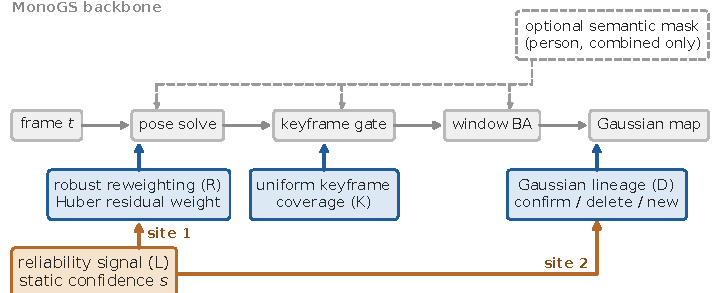
\includegraphics[width=0.73\textwidth]{fig1_pipeline.pdf}
\caption{\emph{Where the components attach.} Grey boxes are the backbone. Blue and orange boxes modify the stage their arrow points into. Dashed grey is the optional semantic mask (combined only, never routed through L) with its three consumers: the mapping loss, the keyframe-insertion gate, and the warm-up-only hard tracking mask of Sec. 5.6. L is consumed at exactly two sites, the pose-solve residual (1) and candidate confirmation in the lifecycle (2).}\end{figure}


\subsection{Coverage: uniform temporal keyframe sampling}


MonoGS selects keyframes adaptively by co-visibility, so density is a property of the scene. Across our five ablation sequences the backbone's native density spans 0.045 to 0.075 keyframes per frame. Coverage adds one rule: more than \texttt{gap\_cap = 5} frames since the last keyframe force an insert, and the native criterion is floored rather than replaced. Density becomes near-constant at 0.198 to 0.204 keyframes per frame, at a cost of 2.7--4.5$\times$ more keyframes and roughly double the map size.


\subsection{Robust reweighting: Huber IRLS inside the pose solve}


R replaces the L2 tracking residual with an iteratively-reweighted least-squares step~\cite{zhang}. For residual $r$ the weight is the standard Huber~\cite{huber} IRLS weight $w_{\text{rob}}(r) = \min(\delta/|r|, 1)$ with $\delta = 0.1$ per channel. It is computed from a detached residual and recomputed at every tracking iteration, so the weights co-adapt with the pose, unlike the fixed per-frame map of Sec. 3.4. A pre-registered ablation (6 sequences spanning five regimes $\times$ 2 alternative kernels $\times$ 3 seeds = 36 runs) supports Huber over the two other M-estimation kernels the codebase implements. Neither is ever better outside the pre-registered floor, and on \texttt{pt2} both degrade clearly, by 1.8 and 2.5 cm.


\subsection{Reliability: a per-frame, per-pixel static-confidence map}


This component consumes optical flow and decides, without any category label, which pixels count as evidence about camera motion (Fig. 2); Fig. 3 shows what this leaves in the final map.


\begin{figure}[t]\centering
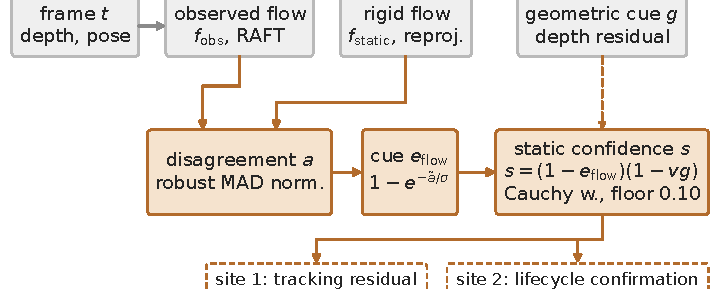
\includegraphics[width=0.76\textwidth]{fig2_reliability.pdf}
\caption{\emph{The reliability signal, from flows to weights (Sec.~3.4).} The observed flow (frozen RAFT) and the rigid reprojection flow disagree on movers. A per-frame robust MAD normaliser turns the disagreement into the cue $e_{\text{flow}}$, which combines with the depth-residual cue $g$ into the static confidence $s$ and the Cauchy tracking weight (floored at 0.10, never removing). The frozen map is consumed at two sites, the tracking residual and lifecycle confirmation.}\end{figure}


\textbf{Observed and rigid flow.} For frame $t$ we take a precomputed backward flow $f_{\text{obs}} = f_{t \to t-1}$ from a frozen RAFT~\cite{raft} network and the rigid-flow prediction $f_{\text{static}}$ from reprojection through the current depth and ego-motion. The mover shows up in that disagreement, though so can occlusion boundaries and flow error, which the robust normaliser of the next step absorbs.


\textbf{Threshold-free normalisation.} The disagreement magnitude becomes a cue $e_{\text{flow}} \in [0,1]$ through the per-frame robust normaliser \texttt{max(1.4826\textperiodcentered{}MAD, floor)}, which maps to 0 at or below the frame median and approaches 1 for robust outliers. The floor (2.0 px) keeps a near-static frame, where MAD collapses, from saturating.


\textbf{Combining the cues.} A geometric cue $g$ measures depth-residual anomaly, gated by opacity $v$ so unmapped regions cannot vote. The two combine into the static confidence $s = (1 - e_{\text{flow}})(1 - vg)$. A pixel is trusted only if both cues find it unremarkable, and $s \to 1$ recovers the unmodified estimator. With $d = 1 - s$ the tracking weight is a frame-adaptive Cauchy down-weight


\begin{equation}
w_{\text{rel}} = \frac{1}{1 + (d/\tau)^2}, \qquad
\tau = \operatorname{median}(d) + 1.4826\,\operatorname{MAD}(d) + \varepsilon
\end{equation}


where the knee $\tau$ is a Hampel-type robust z-score. MAD, the median absolute deviation, is a spread estimate that a minority of outliers cannot move, and the same normaliser that defines $e_{\text{flow}}$ prices deviation from the frame's own $d$ distribution.


\begin{figure}[t]\centering
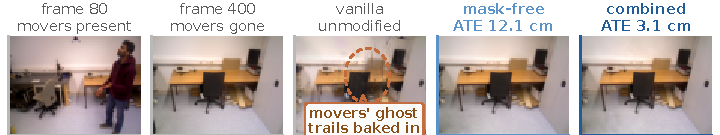
\includegraphics[width=0.68\textwidth]{fig3_map_comparison.pdf}
\caption{\emph{What each configuration bakes into the final map.} Top: the observed scene at frame 80 (person mid-sequence) and at frame 400 after both movers left. Bottom: each arm's final map rendered at frame 400 from its own estimated pose. The backbone's map is shredded by the movers' ghost trails (circled). Both RoGS-SLAM configurations reconstruct the static office, the mask-free one without any class label. The two arms' maps are similar here, since they differ in tracking stability, not map appearance (ATE annotated, Sec. 5.1). Post-hoc offline renders of each run's saved final map, for illustration, not a benchmark metric.}\end{figure}


\textbf{The weight is bounded away from zero.} What multiplies the residual is $\max(w_{\text{rel}}, 0.10)$, so a pixel is attenuated by at most 10$\times$ and never removed. This is the sharpest difference from a mask and the comparison Sec. 5.4 leans on.


\textbf{When it is computed, and where it is consumed.} The map is computed once per frame after \texttt{warmup\_iters = 10} tracking iterations and then frozen. Without frozen flow, $w_{\text{rel}} \equiv 1$ and the estimator is unchanged. It is consumed at two sites. At the \textbf{tracking residual}, $\max(w_{\text{rel}}, 0.10)$ multiplies the Huber weight of Sec. 3.3 in both channels, and at \textbf{candidate confirmation} in the lifecycle of Sec. 3.5, $s$ weights the evidence. The ablation removes this pair of interventions sharing one signal.


\textbf{Where the robust knee breaks.} $\tau$ is a \emph{majority} statistic. A mover occupying a large share of the frame joins the population that sets its own knee, which is one reason the mask stays dominant on mixed-mover sequences (Sec. 5.1).


\subsection{The density lifecycle}


The backbone commits every new Gaussian immediately. Our configuration replaces that commit rule. Each Gaussian created at a keyframe carries a \textbf{lineage} identifier that accumulates support and contradiction evidence. A lineage is retained after 2 units of support (\texttt{confirming\_views}) and deleted in full after 2 units of contradiction (\texttt{reject\_contradictions}) or 5 unconfirmed keyframes (\texttt{ttl\_keyframes}), with $s$ weighting the evidence when reliability is enabled. The replacement is materially active, since the deleted fraction of created lineages has median 0.55. A comparison against stock MonoGS therefore compares a different density rule.


\subsection{The optional semantic mask, and the simpler configuration}


In the \emph{combined} configuration a Mask R-CNN~\cite{maskrcnn} person mask (dilated by 7 px) reaches three consumers: the \textbf{mapping loss}, the \textbf{keyframe-insertion gate}, and the \textbf{tracking residual}. The last is a hard mask only for the first \texttt{warmup\_iters} tracking iterations, after which the soft weight of Sec. 3.4 takes over the person region and the hard mask disengages. The switch between \emph{mask-free} and \emph{combined} opens these paths inside \emph{this} component only, never the reliability signal. Holding the hard mask on for all tracking iterations instead (the single-variable intervention of Sec. 5.6) keeps the hard-excluded region removed while the soft reliability weight continues to apply on surviving static pixels, so the two cues compose rather than replace each other. The attribution campaign uses a third, \emph{simpler} configuration (native sparse keyframes, robust reweighting, the lifecycle, and the mask applied only at the mapping loss) relative to which \emph{combined} flips the three switches of coverage, reliability, and insertion-gate masking. Sec. 5.3 measures the first two in isolation. We report \emph{mask-free}, \emph{combined}, and \emph{simpler} as configurations of one system. All sixteen constants, one of them a disclosed-inert threshold, are resolved from the run configuration.




\section{Experimental Protocol}


Decisions below were frozen before the campaigns of Sec. 5 ran.


\textbf{Sequences.} 18 RGB-D sequences (8 BONN RGB-D Dynamic~\cite{bonn}, 10 TUM RGB-D~\cite{tumrgbd}), spanning static, low-motion, high-motion and \emph{object-only} scenes. The denominator is fixed, no campaign may select a subset after seeing results, and the object-only movers carry no person label.


\textbf{Trajectory accuracy.} Full-trajectory absolute-trajectory error (ATE) RMSE (cm) via \texttt{evo}~\cite{evo} after SE(3) Umeyama alignment~\cite{umeyama} without scale correction. ATE covers all frames, and we also report the relative pose error (RPE, translation, per frame).


\textbf{Seeds and completion.} Every configuration runs with 3 seeds (mean $\pm$ sd, spreads reaching 2$\times$ flagged). A run counts as completed only at $\ge$ 95\% of frames, and a pair with fewer than two co-completed seeds is \emph{unresolved}, not dropped.


\textbf{Rendering, efficiency, hardware.} Rendering metrics are computed offline from the final map, and refinement does not touch the reported trajectory. Efficiency is reported from the online phase and compared only on identical hardware. Flow is precomputed by a frozen RAFT~\cite{raft} network, so RAFT inference is not in the online rate (Sec. 5.7). All campaigns ran on an RTX 3090, and each reported cell maps to exactly one run directory.




\section{Results}


\subsection{Trajectory accuracy under one protocol (Table 1)}


\textbf{On the crowd scenes, combined tracks at 2.3/2.2 cm where the unmodified backbone drifts to 86.5/147.5 cm.} Table 1 compares all reproduced methods on four BONN dynamic scenes. On crowd, combined is the best RGB-D 3DGS configuration (4.4 cm average), although CPU-side NGD-SLAM and DynaSLAM have lower averages of 3.2 and 4.0 cm and produce no dense map. Crowd is the mask-dominant regime (34.9/45.9 cm mask-free). On the object-only scene the segmentation-free arms are unaffected (2.7/3.1), while DynaGSLAM pays for its person-only detector (12.1). On \texttt{pt2}, combined trails WildGS-SLAM (10.4 vs 3.1) and DG-SLAM (6.1), while mask-free is better than combined (9.3).


\begin{table}[t]\centering\scriptsize\setlength{\tabcolsep}{2pt}
\begin{tabular}{>{\raggedright\arraybackslash}p{3.3cm}rrrrrr}\toprule
Method & crowd & crowd2 & mv\_no\_box & pt2 & Avg. & GPU (GB) \\ \midrule
\multicolumn{7}{l}{\emph{Ours, dynamic 3DGS}} \\
RoGS-SLAM combined (ours) & 2.3$\pm$0.0 & 2.2$\pm$0.1 & 2.7$\pm$0.1 & 10.4$\pm$0.8 & 4.4 & 4.0$\pm$1.0 \\
RoGS-SLAM mask-free (ours) & 34.9$\pm$28.3 & 45.9$\pm$17.4 & 3.1$\pm$0.5 & 9.3$\pm$0.6 & 23.3 & 3.4$\pm$1.0 \\
\midrule
\multicolumn{7}{l}{\emph{Dynamic 3DGS}} \\
RGD-SLAM & 2.6$\pm$0.3 & 2.4$\pm$0.1 & 2.3$\pm$0.3 & 23.0$\pm$3.7 & 7.6 & 7.4$\pm$1.1 \\
DG-SLAM & 5.8$\pm$0.1 & 6.4$\pm$0.5 & 3.0$\pm$0.1 & 6.1$\pm$0.1 & 5.3 & 7.3$\pm$0.4 \\
DynaGSLAM & 23.8$\pm$0.0 & 13.7$\pm$0.0 & 12.1$\pm$0.0 & 13.7$\pm$0.0 & 15.8 & 2.2$\pm$0.7 \\
WildGS-SLAM (mono) & {\boldmath$1.55\pm0.06$} & {\boldmath$2.17\pm0.05$} & {\boldmath$1.6\pm0.0$} & {\boldmath$3.1\pm0.0$} & 2.1 & 12.1$\pm$1.9 \\
\midrule
\multicolumn{7}{l}{\emph{Dynamic, non-3DGS}} \\
RoDyn-SLAM (NeRF) & 5.6$\pm$0.2 & 4.6$\pm$0.1 & 16.5$\pm$7.1 & 14.4$\pm$0.1 & 10.3 & 1.0$\pm$0.1 \\
DynaSLAM (CPU) & 2.1$\pm$0.2 & 2.8$\pm$0.3 & 2.3$\pm$0.1 & 8.8$\pm$1.2 & 4.0 & --- \\
NGD-SLAM (CPU) & 1.8$\pm$0.2 & 2.2$\pm$0.1 & 2.0$\pm$0.1 & 6.6$\pm$0.4 & 3.2 & --- \\
\midrule
\multicolumn{7}{l}{\emph{Static}} \\
SplaTAM & 135.4$\pm$36.1 & 493.2$\pm$470.7 & 37.4$\pm$0.4 & 132.7$\pm$9.4 & 199.7 & 6.9$\pm$7.4 \\
MonoGS (unmodified) & 86.5$\pm$18.3 & 147.5$\pm$39.0 & 15.3$\pm$9.5 & 43.8$\pm$8.6 & 73.3 & 0.5$\pm$0.2 \\
Co-SLAM (implicit) & div. & div. & 10.1$\pm$0.3 & 71.3$\pm$2.9 & 40.7 & 1.1$\pm$0.0 \\
ORB-SLAM3 (sparse) & 76.6$\pm$27.9 & 111.4$\pm$14.8 & 24.9$\pm$5.9 & 76.8$\pm$2.1 & 72.4 & --- \\
\bottomrule\end{tabular}
\caption{ATE RMSE (cm, mean $\pm$ sd, 3 seeds) on four BONN dynamic scenes, grouped by representation and dynamic handling. Every row, competitors included, is our own reproduction under one protocol. Reading our rows: \emph{combined} is the full system, \emph{mask-free} its core without the optional semantic mask (Sec. 3.6). \textbf{Bold} marks the lowest ATE per column. Avg and GPU are unranked, since they mix modalities and hardware. div. = diverged. GPU memory: ours and RGD-SLAM share one RTX 3090, the only same-hardware pair. Other rows ran on other hardware and are not comparable across rows. Method citations: Secs.~2.1--2.3.}\end{table}


\textbf{Where the mask matters, measured between our own two arms.} The ratio $N = \text{ATE}_{\text{mask-free}} / \text{ATE}_{\text{combined}}$ never passes through the vanilla denominator, so it is quotable wherever both arms ran. On the six BONN dynamic sequences beyond the crowd pair above, the mask is redundant on \texttt{mv\_no\_box2}, \texttt{mv\_no\_box} and \texttt{pt2} (0.89--1.17$\times$) and dominant on \texttt{balloon2}, \texttt{pt1} and \texttt{balloon} (1.92--3.96$\times$). Sec. 5.5 tracks this split with a per-frame observable across all 18 sequences.


\subsection{Component necessity is regime-dependent (Fig. 4)}


The pre-registered factorial varies K, R, and L (8 cells $\times$ 5 sequences $\times$ 3 seeds = 120 runs). It runs mask-free, with D pinned identically in all cells. Writing the removal effect of component $f$ on sequence $s$ as


\begin{equation}
\Delta_f(s) = E[\log \text{ATE} \mid f \text{ removed}, s] - E[\log \text{ATE} \mid \text{full}, s]
\end{equation}


positive $\Delta_f$ means removing $f$ hurts. Two questions follow: whether any single component is globally necessary ($\Delta_f(s) \ge 0\ \forall s$), and whether any sequence rewards the full bundle ($\Delta_f(s) \ge 0\ \forall f$). With 3 seeds per cell neither question receives an inferential answer, so we apply a descriptive support rule. A cell supports a component only where $|\text{mean}| \ge 1$ sd. Fig.~4 marks a cell that fails the rule with $\circ$, and cells marked $\circ$ are directional, i.e. undetermined rather than negative. Under this rule neither necessity reading is established. $\Delta_L$ is positive on 5 of 5 sequences (the only component with that property, though 3 of the 5 cells are directional), and no sequence has all three components supported (0 of 5), so the full bundle is nowhere strictly necessary across the five measured sequences. Crowd is absent from this factorial. The crowd evidence is the crowd2 ladder of Sec. 5.3.


\begin{figure}[t]\centering
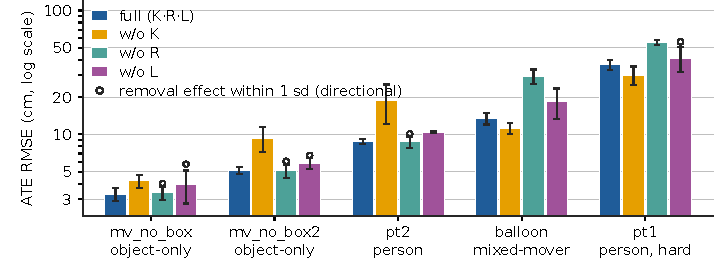
\includegraphics[width=0.68\textwidth]{fig4_component_necessity.pdf}
\caption{\emph{Component necessity is regime-dependent.} For each sequence, ATE RMSE (cm, log scale) of the full mask-free configuration (K$\cdot$R$\cdot$L) and of the three single-component removals, from the pre-registered factorial (8 cells $\times$ 5 sequences $\times$ 3 seeds = 120 runs). Bars are 3-seed means with $\pm$1 sd error bars, and every bar is the factorial's own campaign. Removing coverage ($-$K) raises ATE by 1.3--2.1$\times$ on the three easier sequences yet lowers it on \texttt{balloon} and \texttt{pt1}. Removing robust reweighting ($-$R) is the largest effect in the matrix on \texttt{balloon} (2.2$\times$) and within seed noise on the three easier ones. Removing the reliability signal ($-$L) never helps (5 of 5). $\circ$ marks a removal whose mean log-shift is within 1 sd of its seed spread, i.e. directional only (Sec.~5.2). No sequence rewards all three components (0 of 5).}\end{figure}


$\Delta_K > 0$ strongly on the object-only sequences and \texttt{pt2} yet $\Delta_K < 0$ on \texttt{balloon} and \texttt{pt1}. $\Delta_R$ is not distinguishable from zero at three seeds on the three easier sequences yet is the largest effect in the matrix on \texttt{balloon} (+0.780$\pm$0.037). $\Delta_L$ is the only one never negative (5/5), costing 1.19--1.34$\times$ on \texttt{pt2} and \texttt{balloon}. When L is off, both of its consumption sites go off with it (site 2 reverts to integer counts), so $\Delta_L$ is the joint effect of L's two sites (Sec. 3.4). Two further results belong beside these marginals. A two-by-two ablation over mask and coverage on \texttt{balloon} moves ATE fourfold along the mask axis and not at all along the coverage axis (3.06 vs 3.03 cm), so we do not describe coverage as the kernel. And a cue-split factorial finds geometry-only lower than the shipped fusion on 3 of 4 sequences, so fixed cue fusion is not universal.


\subsection{Single-variable attribution}


The full ladder is descriptive and covers two sequences (24 runs). On \texttt{mv\_no\_box}, coverage alone recovers the full arm's advantage (2.71$\pm$0.04 vs 2.63$\pm$0.09 cm, within the pre-registered floor). On \texttt{crowd2}, no tested subset comes close (coverage 5.16, reliability 6.00, pair 4.55, insertion gating 5.66, full 2.11 cm), so the crowd gain is attributed to the bundle. These cells are attribution-campaign anchors. The 18-sequence denominator reads 2.19$\pm$0.09 (crowd2) and 2.65$\pm$0.12 (mv\_no\_box), inside the drift discipline (we budget $\sim$30\%: audited same-configuration anchors have moved by up to $\sim$15\% between campaigns, and a same-seed re-run by 1.36$\times$), and the 18-sequence campaign is canonical.


\subsection{The gain is not the flow information alone (Fig. 5a)}


To isolate the gain from the information, the counterpart consumes the same frozen backward flow, byte for byte, through a naive p90 threshold (frozen on pilot sequences) as a hard mask in place of our weighting. The control comprises 3 arms $\times$ 4 sequences $\times$ 3 seeds = 36 runs, rule fixed before the first.


The naive counterpart stably beats vanilla on only 2 of 4 under the all-seeds-same-sign rule and is worse on \texttt{pt2} (51.07 vs 45.37 cm, a 1.13$\times$ flow-mask/vanilla ratio). Ours improves on all four (1.63--4.99$\times$) and beats the counterpart on all four. Every cell here, vanilla included, comes from the control's own campaign. The 18-sequence campaign's vanilla on \texttt{pt2} reads 43.85$\pm$8.55, a cross-campaign gap inside the drift discipline of Sec. 5.3, and ratios here divide same-campaign cells. The counterpart also lacks the MAD normaliser and geometric cue and uses hard removal, so the control rules out the information alone, not every flow-consuming treatment.


\subsection{Where mask-free stops being sufficient (Fig. 5b)}


We test whether the mask-free arm's own per-frame RPE tracks that split. Across all 18 sequences, necessity is read as $N$ ($N \ge 1.5$ necessary, $N \le 1.2$ redundant).


The groups do not overlap, spanning 0.222--1.572 against 1.717--2.980 cm/frame. Every threshold in between separates all 17 decided sequences. \texttt{f3\_st\_hf} and \texttt{crowd} have nearly identical mask-free ATE yet $N$ values differing 12.6-fold. Per-frame drift tracks mask necessity, and accumulated error does not.


\begin{figure}[t]\centering
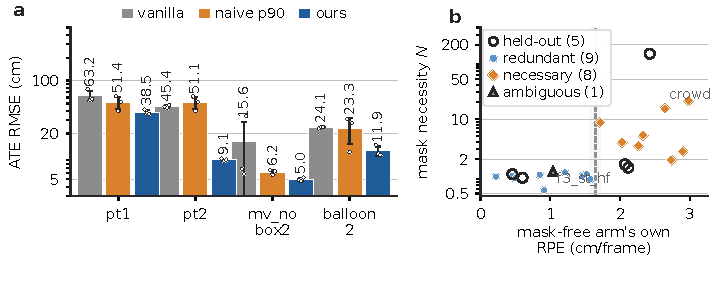
\includegraphics[width=0.68\textwidth]{fig5_controlled_comparison.pdf}
\caption{\emph{Two controlled comparisons.} (a) Flow-budget counterpart (Sec.~5.4): ATE RMSE (cm, log scale) when the same byte-identical frozen flow is consumed by nothing (vanilla), a naive p90 threshold, or our weighting. Dots are seeds, bars are 3-seed means ($\pm$1 sd). On \texttt{pt2} the naive threshold is worse than vanilla (51.1 vs 45.4~cm) while ours is 5.0$\times$ better, and ours stays below parity on all 12 seeds. (b) Mask necessity $N$ against the mask-free arm's own per-frame RPE (Sec.~5.5). The two groups do not overlap. The grey band is the empirical gap and the dashed line is the pre-registered midpoint $\tau$. Black-edged markers are the first-round held-out checks (5), of which four agree and one lands in the band, undecidable.}\end{figure}


\textbf{Scope of the interval.} The interval requires running the mask-free arm, which makes it a post-hoc diagnosis rather than a selector. Its pre-registered midpoint ($\tau = 1.6445$ cm/frame) was tested on two rounds of unseen sequences (5, then 6, all outside the denominator). The ambiguity band is the open interval $(1.2, 1.5)$, and $N \le 0.8$ is the frozen-sense line. One first-round sequence lands in the band, undecidable, so 10 remain. Eight of the 10 agree in direction (4 of 4 decidable in round one, the black-edged points in Fig.~5b with one in-band, and 4 of 6 in round two), and both misses are conservative. No RPE fell inside the band, whose location is untested.


\subsection{The pose-side mechanism}


\begin{figure}[b]\centering
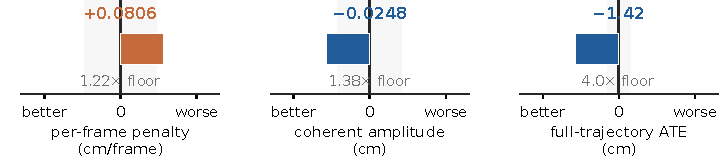
\includegraphics[width=0.85\textwidth]{fig6_pose_endpoints.pdf}
\caption{\emph{One intervention, three pose-side endpoints, opposite signs (Sec.~5.6).} Shift on \texttt{balloon} from holding the semantic hard tracking mask on for all 100 tracking iterations instead of 10 (intervention minus control, raw units per endpoint, grey band $\pm$1 re-run noise floor of that endpoint). The per-frame dynamic penalty moves worse ($+0.0806$ cm/frame, $1.22\times$ floor), the coherent amplitude lower ($-0.0248$ cm, $1.38\times$), and full-trajectory ATE better ($-1.42$ cm, $4.0\times$). This is the variance--bias trade of Sec.~5.6, measured on one sequence with two legs near their floors.}\end{figure}


One intervention holds the semantic hard tracking mask of combined on for 100 tracking iterations instead of 10, with soft reliability retained on surviving static pixels. It changes three pose-side endpoints (Fig.~6). The \emph{per-frame dynamic penalty}, median RPE on high-dynamic frame pairs minus median RPE on low-dynamic pairs (cm per frame), moves worse (+0.0806, 1.22$\times$ floor). The \emph{coherent amplitude}, mean cosine similarity between consecutive RPE vectors times median $|$RPE$|$ on the high-dynamic pairs (cm), moves lower ($-$0.0248, 1.38$\times$). Full-trajectory ATE moves better ($-$1.42 cm, 4.0$\times$). The measurement is consistent with a variance--bias trade but rests on \texttt{balloon} alone, two legs near their floors. Writing $e_t=b_t+\varepsilon_t$ with zero-mean $\varepsilon_t$, suppressing pixels can raise per-frame noise while lowering the systematic pull that accumulates into drift. A tracking claim must therefore name its endpoint.


\subsection{Rendering and cost}


Combined runs at 0.75$\pm$0.09 FPS and 4.02$\pm$1.01 GB on the same RTX 3090, within one sd of mask-free (0.77$\pm$0.21, 3.43$\pm$0.99). Mask R-CNN runs online, cached per keyframe, and precomputed RAFT (54 ms/frame) is excluded. Across 18 sequences, post-hoc renders show full-frame PSNR ranking the ghost-carrying backbone above both arms (19.1 vs 18.8/18.6 dB), so PSNR is read as map self-consistency, never trajectory evidence. Depth-L1, the one rendering metric co-ordered with ATE, improves from 46.9 to 31.4--32.3 cm, a geometry gain usable downstream.




\section{Limitations}


\textbf{1. Where our arms lose.} On \texttt{pt1}, mask-free reaches 32.41$\pm$8.52 cm against the mask's 11.89$\pm$2.36 (\texttt{pt2} needs no mask). On four of the 18 sequences both arms are worse than the backbone: \texttt{f3\_st\_hf} an order of magnitude (35.59/29.43 vs 2.80 cm), the others 1.1--2.8$\times$ (the \texttt{f3\_st\_hf} exception is recoverable, to 2.67$\pm$0.27 cm at a larger async budget).


\textbf{2. Accuracy scope.} Combined trails the best RGB-D comparator by 1.0--1.7$\times$ on the walking and person sequences (\texttt{f3\_wk\_hf} 3.29 vs 3.25 for RGD-SLAM and \texttt{pt2} 10.45 vs 6.1 for DG-SLAM), and monocular WildGS-SLAM by 3.4$\times$ on \texttt{pt2}.


\textbf{3. Static scenes.} On Replica~\cite{replica}, outside the denominator, combined is worse and less stable than the backbone (\texttt{office0} 3.82$\pm$4.58 vs 0.368$\pm$0.012 cm), so use it only when no dynamic content is present.


\textbf{4. Operating conditions.} On 8/18 sequences baseline CV exceeds 20\%, making ratios basin-dependent (Sec. 4).


\textbf{5. Crowd attribution and scope.} The crowd gain is attributable to the bundle, since no single component recovers it (Sec. 5.3, descriptive). Evidence comes from one MonoGS implementation, and semantic area, the simplest cue selector tested, does not separate the regimes.




\section{Conclusion}
% Final content page sits 3 lines past the 12-page boundary and the llncs
% widow/club penalties (10000) lock the Conclusion paragraph's break point.
% A one-page enlargement of 4 lines closes the gap; same technique the
% bibliography already uses (main_v3.tex uses 12\baselineskip there).
\enlargethispage{4\baselineskip}


We presented RoGS-SLAM, a mask-free core for dynamic 3DGS-SLAM, and the measurements that bound it: component necessity is regime-dependent, the gain does not follow from the information alone, and pose-side claims must name the endpoint. The regime split holds within the stated limits, the RPE separation stays post-hoc, and a mask-free cue selector is future work.



